\documentclass[12pt]{article}
%packages
\usepackage{tikz}
\usetikzlibrary{mindmap}

\begin{document}
%create more creative we use mindmap, here we define tikzpicture environment.
%here we define style in each and every node
%concept is the way in which your figure will look like
%here we use append style for both the lavels
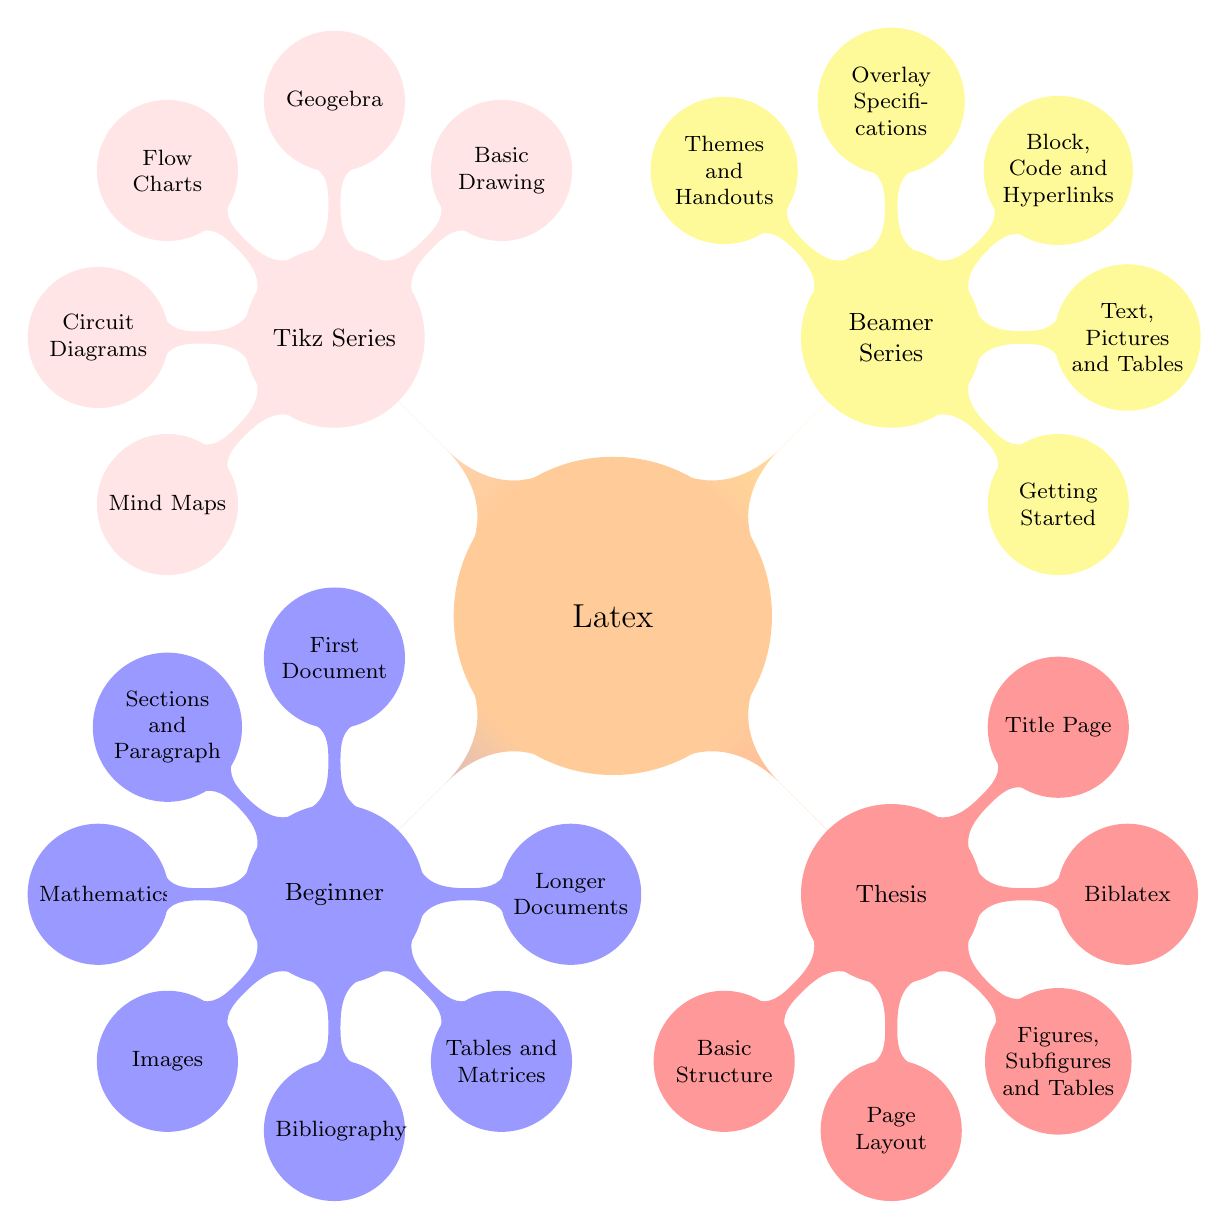
\begin{tikzpicture}[mindmap, grow cyclic, every node/.style=concept, concept color=orange!40,
	level 1/.append style={level distance=5cm, sibling angle=90},
	level 2/.append style={level distance=3cm, sibling angle=45},]  %to create more creative
	
	%or (below style is not very creative)
	%here we define style for whole diagram
%\begin{tikzpicture}[grow cyclic, text width=2.7cm, align=flush center, %grow cyclic means you trying to create cyclic type of diagram, %create levels to omit overlapping
%	level 1/.style={level distance=5cm, sibling angle=90}, % here we create level 1 because here we have 4 children..beginner, thesis, beamer series, tikx series,
%	level 2/.style={level distance=3cm, sibling angle=45}] %here we create level 2 because each child hast different children. % select angle as your convaniant
 \node{Latex} %main node
	%different children nodes
	child {[concept color=blue!40]  node {Beginner}
         child {node {First Document}}
         child {node {Sections and Paragraph}}
	     child {node {Mathematics}}
	     child {node {Images}}
	     child {node {Bibliography}}
	     child {node {Tables and Matrices}}
	     child {node {Longer Documents}}
	  }
	child {[concept color=red!40] node {Thesis}
         child {node {Basic Structure}}
		 child {node {Page Layout}}
	     child {node {Figures, Subfigures and Tables}}
	     child {node {Biblatex}}
	     child {node {Title Page}}
	}
	child {[concept color=yellow!40] node {Beamer Series}
		 child {node {Getting Started}}
		 child {node {Text, Pictures and Tables}}
	     child {node {Block, Code and Hyperlinks}}
		 child {node {Overlay Specifications}}
	     child {node {Themes and Handouts}}
	}
	child {[concept color=pink!40]  node {Tikz Series}
         child {node {Basic Drawing}}
		 child {node {Geogebra}}
	     child {node {Flow Charts}}
	     child {node {Circuit Diagrams}}
	     child {node {Mind Maps}}
	}
;

\end{tikzpicture}

\end{document}




